\chapter{Metodología para la generación de fuentes Monte Carlo mediante histogramas multidimensionales}
\label{cap:metodo_histogramas}
\section{Introducción general al método}
La metodología propuesta se basa en el procesamiento de archivos de partículas generados en simulaciones Monte Carlo previas, específicamente usando \texttt{OpenMC}, para definir fuentes distribucionales para simulaciones subsiguientes.

\section{Definición del espacio de fases \texorpdfstring{$(\mathbf{E}$--$\mathbf{r}$--$\boldsymbol{\Omega})$}{(E--r--Omega)}}
Para aproximar correctamente las distribuciones y correlaciones del espacio de fases se consideraron seis variables para representar la energía, posición y dirección: tres coordenadas espaciales $(x, y, z)$, dos variables direccionales definidas en coordenadas esféricas ($\mu = \cos(\theta), \phi$) y una variable energética ($E$ o letargía $ln(E_0/E)$). En la Figura \ref{fig:terna} se observa una representación de las variables del espacio de fases. En situaciones como la considerada en este trabajo, donde la fuente se registra sobre una superficie plana, es posible rotar el sistema de coordenadas de modo que dicha superficie resulte perpendicular al eje $z$. Por lo tanto la coordenada $z$ permanece constante, permitiendo representar el espacio de fases con cinco variables.

\begin{figure}[h]
    \centering
    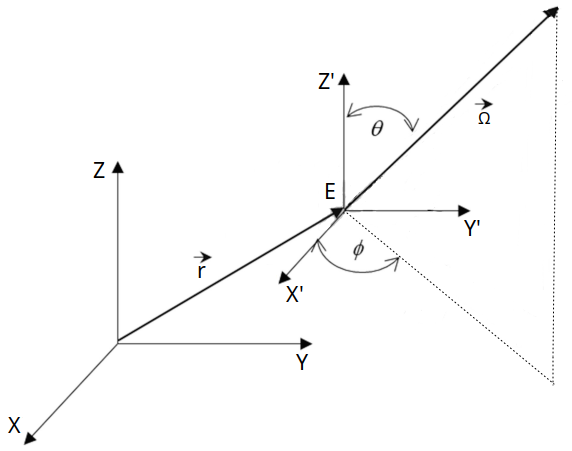
\includegraphics[width=0.5\textwidth]{figs/terna.png}
    \caption{Representación del espacio de fases con las variables $(E, x, y, z, \theta, \phi)$, donde $E$ es la energía, $x$, $y$ y $z$ son coordenadas espaciales y $\theta$ y $\phi$ son las variables direccionales.}
    \label{fig:terna}
\end{figure}

\section{Procesamiento del archivo de partículas original}
\subsection{Preprocesamiento del archivo de partículas}
Inicialmente, las partículas provenientes de la simulación Monte Carlo original se filtran seleccionando únicamente aquellas que se propagan hacia la región de interés y se separan las variables relevantes mencionadas, además del peso estadístico (\textit{weight}). Esta selección se realiza porque, en la siguiente etapa de simulación, la geometría considera un vacío en la región donde originalmente se encontraba la superficie de registro, permitiendo que únicamente las partículas que avanzan en dirección hacia la región de interés puedan ser simuladas. Las partículas que se dirigen en sentido opuesto no son relevantes para la simulación posterior, ya que en caso de que alguna partícula inicialmente dirigida hacia atrás fuese a regresar por retrodispersión, dicho comportamiento ya está estadísticamente incorporado en la lista original de partículas, producto de la simulación completa previa. En la Tabla \ref{tab:estructura_trackfile} se presenta un ejemplo de la estructura típica de un archivo de partículas.

\begin{table}[h]
    \centering
    \begin{tabular}{ccccccc}
        \toprule
        \textbf{Partícula Nº} & \textbf{Letargía} & \textbf{x [cm]} & \textbf{y [cm]} & \textbf{$\mu$} & \textbf{$\phi$ [rad]} & \textbf{Peso estadístico} \\ 
        \midrule
        1       & 4.15 &  0.23  & -1.10 &  0.85 & 3.14 & 1.00 \\
        2       & 4.95 & -0.75  &  0.40 & 0.65 & 1.57 & 1.00 \\
        3       & 5.05 &  1.10  &  0.70 &  0.45 & 0.78 & 1.00 \\
        4       & 5.30 & -0.50  & -0.90 &  0.60 & 2.35 & 1.00 \\
        5       & 4.85 &  0.85  & -0.20 & 0.95 & 1.25 & 1.00 \\
        $\vdots$ & $\vdots$ & $\vdots$ & $\vdots$ & $\vdots$ & $\vdots$ & $\vdots$ \\[0.2cm]
        100000  & 5.00 &  0.10  &  0.55 & 0.70 & 0.95 & 1.00 \\
        \bottomrule
    \end{tabular}
    \caption{Ejemplo ilustrativo de la estructura típica de un archivo de partículas. El archivo original suele contener cientos de miles de partículas.}
    \label{tab:estructura_trackfile}
\end{table}

\subsection{Utilización de histogramas macro y micro}
La metodología desarrollada en este trabajo para aproximar distribuciones y correlaciones multidimensionales en el espacio de fases de partículas provenientes de simulaciones Monte Carlo se basa en un esquema combinado de histogramas macro y micro. Esta aproximación permite gestionar eficientemente grandes volúmenes de datos manteniendo una representación precisa de la información esencial del conjunto original de partículas.

Los histogramas macro son subdivisiones jerárquicas del espacio de fases, realizadas siguiendo un orden determinado por el usuario. Por ejemplo, un posible orden es la \textit{letargía}, seguida por las coordenadas espaciales (\textit{X}, \textit{Y}), y posteriormente por la dirección (\textit{$\mu$}, \textit{$\phi$}). Este procedimiento inicia dividiendo el conjunto original de partículas en macrogrupos según la primera variable elegida (por ejemplo, \textit{letargía}). Cada macrogrupo así generado es posteriormente subdividido en nuevos macrogrupos en función de la siguiente variable (por ejemplo, la coordenada \textit{X}), repitiéndose este proceso de manera iterativa para cada variable subsiguiente. El resultado es una estructura jerárquica en forma de árbol, donde cada rama representa un subconjunto específico del archivo original de partículas, ya que incluye las cinco variables consideradas. Cada nodo en la rama corresponde a  una variable dentro de dicho subconjunto. En la Figura \ref{fig:estructura_jerarquica} se ilustra este procedimiento de subdivisión jerárquica del espacio de fases.

\begin{figure}[h]
    \centering
    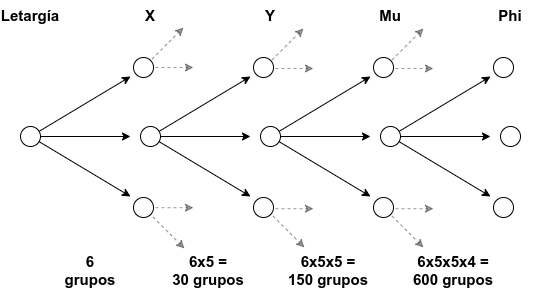
\includegraphics[width=0.8\textwidth]{grupos.png}
    \caption{Esquema ilustrativo de la estructura jerárquica de macrogrupos y microgrupos formando un árbol. Se resalta claramente la jerarquía entre variables.}
    \label{fig:estructura_jerarquica}
\end{figure}

Este esquema tiene como objetivo capturar las correlaciones entre las variables del espacio de fases. Cada nodo o macrogrupo resultante comparte similitudes en todas las variables consideradas hasta ese nivel jerárquico. Por ejemplo, un macrogrupo particular tendrá partículas con distribuciones similares en \textit{letargía}, coordenadas espaciales (\textit{X}, \textit{Y}), y dirección \textit{($\mu$)}, lo cual garantiza que la distribución restante en la última variable \textit{($\phi$)} refleje adecuadamente las correlaciones subyacentes en los datos.

Cabe destacar que, en la etapa de macrodiscretización, se utilizan histogramas con baja resolución debido al crecimiento exponencial en la cantidad total de grupos generados, dado que el número total de macrogrupos es producto del número de divisiones en cada variable. Un número excesivamente alto de divisiones podría conducir a subconjuntos con muy pocas partículas, comprometiendo la calidad estadística.

Una vez establecidos los macrogrupos, cada nodo es discretizado con histogramas micro, los cuales poseen una mayor resolución para representar detalladamente la distribución de cada variable dentro del subconjunto. Sin embargo, es crucial controlar esta resolución para evitar reproducir el ruido estadístico presente en los datos originales, especialmente cuando se cuenta con un número reducido de partículas en el subconjunto.

La combinación de histogramas macro y micro permite obtener una aproximación eficiente y precisa de la distribución multidimensional del conjunto original, conservando las correlaciones entre las variables del espacio de fases. Esta estructura de histogramas multidimensionales representa, en síntesis, la información esencial extraída del archivo original de partículas para ser utilizada en simulaciones posteriores.

\subsection{Métodos de discretización aplicados a histogramas macro y micro}
En este trabajo se desarrollaron dos métodos de discretización (bineado) aplicables tanto a los histogramas macro como a los micro. El primero es el \textit{bineado uniforme}, que consiste en dividir la distribución de la variable en estudio utilizando bines equiespaciados. Este método tiene la ventaja de ser sencillo y rápido en su implementación, pero presenta la desventaja de no poder capturar adecuadamente cambios abruptos o picos aislados en las distribuciones.

El segundo método, denominado \textit{bineado adaptativo}, consiste en realizar inicialmente un bineado uniforme con una cantidad moderada de bines especificada por el usuario. Luego, este bineado inicial se refina iterativamente agregando nuevos bines donde la distribución estimada difiere en mayor medida respecto a la distribución original. El criterio para añadir un nuevo bin se basa en la comparación de la función de distribución acumulada (FDC) del bineado actual con la FDC de la distribución original calculada con alta resolución. En cada iteración, se identifica el punto con la mayor diferencia absoluta entre ambas FDC, donde se coloca un borde de bin adicional. En el \textbf{Apendice B} se presenta un ejemplo de la implementación de este método.

Este enfoque adaptativo permite asignar mayor resolución donde existe una mayor cantidad de peso estadístico, y menor resolución donde el peso es escaso, logrando así un mejor seguimiento de las zonas críticas y un adecuado suavizado en regiones con poca estadística.

Además, debido a que la cantidad de partículas generalmente disminuye al profundizar en las ramas del árbol jerárquico, puede ser necesario utilizar una resolución decreciente en las discretizaciones, tanto para los histogramas macro como para los micro, lo cual también ha sido implementado en este trabajo.

Finalmente, en aquellos casos en que el usuario conozca previamente la existencia de cambios abruptos o picos específicos en la distribución, es posible informar manualmente al método sobre la ubicación de estos fenómenos, estableciendo bordes de bin específicamente en esos puntos para mejorar la precisión de la discretización.


% \section{Aproximación de distribuciones mediante histogramas micro}

% Las distribuciones de las variables en el espacio de fases pueden representarse, de forma general, mediante histogramas. La elección del método de discretización (bineado) es crucial y condiciona la calidad de la aproximación obtenida. Los tres esquemas de bineado utilizados en este trabajo son:

% \begin{itemize}
%     \item \textbf{Bineado de igual separación}: Divide el rango completo de la variable en intervalos de ancho constante. 

%     \item \textbf{Bineado de igual integral}: Divide el rango en intervalos que contienen aproximadamente la misma cantidad de peso estadístico, generando así bines de tamaño variable. Este método logra una representación más eficiente en términos estadísticos, especialmente en regiones donde la densidad cambia abruptamente.

%     \item \textbf{Bineado adaptativo}: Divide el rango utilizando una discretización iterativa que asigna mayor resolución a las zonas de alta densidad estadística y menor resolución en regiones escasamente pobladas, con el objetivo explícito de reducir el ruido estadístico manteniendo manteniendo resolución en los cambios abruptos de la distribución.
% \end{itemize}

% En este trabajo se profundiza particularmente sobre el método de bineado adaptativo. El procedimiento propuesto se realiza en dos etapas principales:

% \begin{enumerate}
%     \item \textbf{Aproximación inicial gruesa}: Se discretiza la distribución con una cantidad reducida de bines uniformemente distribuidos, típicamente utilizando cerca del 25\% del número final previsto de bines, aunque puede ser definido por el usuario.
    
%     \item \textbf{Refinamiento iterativo}: En cada iteración se evalúa la diferencia absoluta entre la distribución acumulada estimada (FDC) aproximada mediante los bines actuales y la FDC de referencia calculada con muchos bines. Se agregan bines adicionales precisamente en las regiones donde esta diferencia es máxima, mejorando progresivamente la calidad del histograma resultante.
% \end{enumerate}

% Esta estrategia adaptativa permite capturar adecuadamente las regiones críticas de la distribución, proporcionando un balance controlado entre resolución local y suavidad global.

% \section{Aproximación de distribuciones mediante histogramas adaptativos}
% La distribución de cada variable es representada mediante histogramas con bines de ancho no uniforme, seleccionados mediante una técnica de \textit{binning} adaptativo. Este procedimiento asigna mayor resolución a regiones del espacio de fases con mayor densidad estadística y menor resolución en regiones de baja estadística, con el fin de reducir el ruido estadístico.

% El proceso adaptativo se realiza en dos etapas principales:
% \begin{enumerate}
%     \item Una aproximación gruesa con una cantidad inicial de bines uniformes (aproximadamente el 25\% del total).
%     \item Ajuste iterativo agregando nuevos bines donde la diferencia absoluta entre la distribución acumulada estimada (CFD) y la distribución acumulada real (calculada con un gran número de bines) es mayor.
% \end{enumerate}


% \section{Mantenimiento de correlaciones mediante histogramas macro}

% El algoritmo desarrollado permite preservar las correlaciones entre variables del espacio de fases a través de divisiones sucesivas del conjunto de datos. Este proceso admite tres esquemas posibles de bineado para cada variable: de igual separación, de igual integral o adaptativo. En todos los casos, la variable considerada se utiliza para dividir el conjunto de partículas actual en subgrupos o \emph{macrogrupos}, que son luego tratados recursivamente.

% Particularmente, en el caso del bineado adaptativo, el procedimiento comienza con una partición inicial de baja resolución distribuidos uniformemente y se aplica un refinamiento iterativo utilizando un criterio similar al empleado en la sección anterior: se identifican las regiones donde la separación entre la distribución acumulada empírica y la distribución acumulada de referencia es mayor, y se subdividen esas regiones para aumentar la resolución local.

% Este proceso de partición se aplica a cada variable en un orden definido por el usuario, generando una estructura en forma de árbol. En cada nodo del árbol se almacena la distribución acumulada de la variable correspondiente a ese nivel, junto con las fronteras de los macrogrupos definidos. Esta estructura permite preservar las correlaciones multidimensionales entre variables, ya que cada división se realiza condicionada a las divisiones previas.


% \section{Mantenimiento de correlaciones mediante macrogrupos}
% Para preservar la correlación entre variables, se utiliza una estrategia basada en la división secuencial del conjunto de datos en macrogrupos, comenzando con una división gruesa en cuatro subconjuntos y luego refinándola iterativamente mediante el procedimiento adaptativo hasta alcanzar la cantidad deseada de macrogrupos.

% Este proceso jerárquico y secuencial se aplica iterativamente a cada una de las variables del espacio de fases, dando lugar a una estructura de árbol donde cada nodo contiene información sobre la distribución acumulada de la variable correspondiente.

% En la figura \ref{fig:estructura_jerarquica} se muestra un esquema ilustrativo de la distribución jerárquica en macrogrupos. En este caso, la letargía constituye la primera variable que se procesa y se subdivide en distintos macrogrupos en la variable X. A continuación, cada uno de estos macrogrupos en X es nuevamente dividido en macrogrupos en la variable Y. Este procedimiento se repite para las variables subsiguientes, como Y y $\mu$. De este modo, cada nodo en la estructura representa un subconjunto específico del archivo de particulas original. Posteriormente, cada subconjunto es aproximado mediante un histograma micro, permitiendo obtener una estimación detallada de la distribución asociada a ese subconjunto.



\section{Remuestreo de partículas en simulaciones Monte Carlo subsecuentes}
El proceso de generación de partículas a partir de la información guardada en los histogramas multidimensionales implica:
\begin{enumerate}
    \item Generar un número pseudoaleatorio entre 0 y 1.
    \item Interpolar dicho número en la distribución acumulada normalizada de la variable raíz del árbol.
    \item Avanzar secuencialmente por las ramas del árbol determinando valores de las variables subsecuentes hasta obtener un conjunto completo de variables del espacio de fases.
\end{enumerate}

En la Figura \ref{fig:esquema_generacion_particulas} se ejemplifica el proceso de generación de partículas descrito previamente. En el caso particular de trabajar con cinco variables, se repetirá la generación de números pseudoaleatorios cinco veces consecutivas, obteniéndose así los cinco valores correspondientes de las variables. Cabe destacar que durante el remuestreo de la quinta variable no se generará un macrogrupo adicional, dado que esta es la última variable a muestrear y no existen más niveles en el árbol.

\begin{figure}[H]
    \centering
    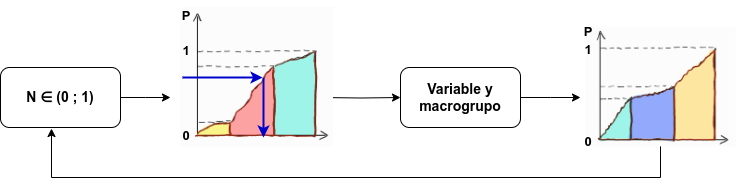
\includegraphics[width=\textwidth]{esquema5.png}
    \caption{Esquema ilustrativo del proceso secuencial de generación de partículas a partir de la distribución jerárquica guardada, resaltando el muestreo sucesivo mediante números pseudoaleatorios.}
    \label{fig:esquema_generacion_particulas}
\end{figure}

% Este enfoque evita la necesidad de cargar grandes listas en memoria \textit{RAM} durante la ejecución de simulaciones Monte Carlo, lo que simplifica considerablemente el manejo de fuentes en \texttt{OpenMC}.

% Este enfoque permite generar partículas para una siguiente simulación Monte Carlo. 

A través de este proceso es posible remuestrear nuevas partículas para la siguiente etapa de la simulación. Existen dos formas de integrar esta funcionalidad con \texttt{OpenMC}:

\begin{itemize}
    \item Una opción consiste en realizar, de forma \emph{offline}, el muestreo de una cantidad predeterminada de partículas y guardar sus propiedades en un archivo de partículas. Este archivo puede ser luego utilizado por \texttt{OpenMC} mediante su opción de simulación desde el modo de fuente \textit{FileSource} implementado en el programa.
    
    \item Alternativamente, se puede ejecutar \texttt{OpenMC} con una fuente del tipo \texttt{HistogramSource}, definida \textit{ad hoc} y configurada mediante un archivo \texttt{XML}. En este caso, \texttt{OpenMC} accede directamente al árbol de histogramas durante la simulación y genera cada partícula \emph{on-the-fly}, lo que reduce significativamente el uso de memoria y evita la necesidad de almacenar archivos de partículas intermedios voluminosos.
\end{itemize}

Esta funcionalidad fue incorporada en el contexto del presente trabajo, mediante la definición de una nueva clase de fuente en el código fuente de \texttt{OpenMC} en \texttt{C++}. Se desarrollaron las estructuras necesarias en \texttt{C} para efectuar el muestreo desde histogramas multidimensionales, y se integraron con la \texttt{API} de \texttt{OpenMC} en \texttt{Python}, permitiendo así que los histogramas puedan ser cargados y utilizados dentro del flujo habitual de simulación. El objetivo principal de esta implementación es facilitar el uso práctico de la herramienta.


\section{Implementación computacional}

La implementación computacional de la metodología descrita en este capítulo se encuentra desarrollada y documentada en el \textbf{Apendice A}. En particular, se presentan los códigos elaborados en \texttt{Python}, \texttt{C} y \texttt{C++} que posibilitan la generación y manejo de los histogramas multidimensionales generados a partir del archivo original de particulas. Dichos histogramas se configuran mediante parámetros específicos definidos por el usuario, tales como número y tipo de bines, así como el orden en que se procesan las variables del espacio de fases.

Asimismo, se documenta en detalle la integración realizada con \texttt{OpenMC}, incluyendo las modificaciones llevadas a cabo en su \textit{API} de \texttt{Python} y en su código fuente en \texttt{C++}, para permitir la generación \textit{on-the-fly} de partículas durante las simulaciones Monte Carlo subsecuentes.



% \section{Implementación computacional}
% La metodología descrita para estimar las distribuciones y correlaciones del \textit{trackfile} ha sido implementada en \texttt{Python}, debido a su leve/moderado costo computacional, creando una rutina que permite configurar parámetros tales como el número de bines y tipo de bineado para los histogramas macro y micro para cada variable, como así también el orden de procesamiento de las mismas. Esta rutina también ofrece la opción de insertar bordes manuales en los histogramas macro cuando se dispone de información previa que optimice la estimación.

% La estructura generada (árbol jerárquico de histogramas multidimensionales) es almacenada en un archivo \texttt{XML}, formato ideal debido a la estructura tipo árbol del dato generado. Posteriormente, esta información es utilizada directamente como fuente en simulaciones Monte Carlo subsecuentes en \texttt{OpenMC}, mediante modificaciones específicas realizadas tanto en su \textit{API} de \texttt{Python} como en su código fuente en \texttt{C++}.

% % \section{Conexión con la implementación computacional}
% La metodología expuesta fue implementada mediante códigos desarrollados en \texttt{Python}, \texttt{C} y \texttt{C++}, integrados específicamente dentro de los entornos de simulación Monte Carlo \texttt{OpenMC} y \texttt{KDSource}. La implementación detallada y comentada de estos códigos se presenta en el \textbf{Anexo A}, mostrando de forma explícita cómo se lleva a la práctica el proceso descrito anteriormente.

% En los capítulos siguientes el desempeño del método descrito será evaluado para cuantificar el grado en que el método conserva las propiedades originales del \textit{trackfile} registrado.
